\documentclass[10pt,conference]{IEEEtran}

\usepackage{amsmath,amssymb}
\usepackage{booktabs}
\usepackage{graphicx}
\usepackage{microtype}
\usepackage{url}
\usepackage{cite}

\begin{document}

\title{One Trellis, Two Assessments: An Embedded CTC--Viterbi Alternative to MFA for Phoneme and Lexical-Stress Scoring}

\author{\IEEEauthorblockN{Long, Nguyen Trung}
\IEEEauthorblockA{\texttt{long.nt270504@gmail.com}}}

\maketitle

\begin{abstract}
Pronunciation-assessment systems often run an external forced aligner before
computing phoneme goodness and syllable-stress features. We investigate whether
one resident phoneme Connectionist Temporal Classification (CTC) model can do
both jobs. Our system decodes the maximum-probability path through a canonical
phone-conditioned CTC trellis, uses phone-state frames for mean log-posterior
scores, and converts the same path into continuous regions for a fixed
Mallela-inspired sequential stress scorer. Montreal Forced Aligner (MFA) 3.4.2
is the external-alignment baseline. In a controlled SpeechOcean762 experiment,
the CTC and MFA conditions share the acoustic posteriors, targets, score,
calibration, and stress model; only phone-region estimation differs. On 43,613
paired test phones, CTC--Viterbi obtains calibrated Pearson correlation 0.459
versus 0.317 for MFA. The paired difference is 0.142 (95\% speaker-bootstrap
confidence interval 0.120--0.164). On 1,575 polysyllabic words whose human
stress grade is correct, canonical stress-location accuracy is 74.9\% versus
69.5\%, a 5.4-point difference (95\% interval 2.8--8.0). A complete paired
batch---one CTC encoding, 43,613 phone scores, and 1,621 polysyllabic stress
predictions per condition---takes 98.6 ms per utterance with CTC--Viterbi and
128.8 ms with a one-job MFA baseline, a 1.31$\times$ speed ratio. The results
support an MFA-free architecture without an observed accuracy trade-off under
this protocol.
\end{abstract}

\begin{IEEEkeywords}
pronunciation assessment, goodness of pronunciation, CTC, Viterbi decoding,
lexical stress, forced alignment
\end{IEEEkeywords}

\section{Introduction}

Computer-assisted pronunciation training benefits from both segmental
feedback---which phone was weak---and suprasegmental feedback---which syllable
received lexical stress. Classical goodness-of-pronunciation (GOP) systems
first align a known transcript and then aggregate acoustic-model evidence
inside each phone interval~\cite{witt2000phone,hu2015improved}. Stress systems
likewise require temporal regions because duration, intensity, pitch, and
sonority are properties of a syllable or its nucleus rather than a complete
utterance~\cite{fry1958experiments,yarra2019comparison}.

Montreal Forced Aligner (MFA) provides reliable, general-purpose word and phone
intervals through a Kaldi-based alignment pipeline~\cite{mcauliffe2017montreal,
povey2011kaldi}. It also introduces a second acoustic model, a pronunciation
dictionary, a database, subprocess orchestration, and a handoff of alignment
artifacts. Those costs are reasonable for corpus preparation but unattractive
for an interactive tutor already running a phoneme CTC model.

This work asks whether the resident CTC model can supply the necessary phone
regions itself. CTC was designed to train sequence models without frame-level
labels by marginalizing paths that collapse to an output sequence
~\cite{graves2006connectionist}. At inference, the same topology supports a
maximum-probability path constrained by the expected phone sequence. We call
this operation \emph{embedded CTC--Viterbi alignment}. It is not unconstrained
phone recognition: the canonical phones define the trellis. The architectural
claim is narrower and operational: no external MFA/Kaldi alignment job is used
by an assessment request.

Figure~\ref{fig:architecture} contrasts the two pipelines. Our contributions
are:
\begin{itemize}
    \item a tested CTC--Viterbi decoder whose phone regions drive both phoneme
    scoring and lexical-stress features;
    \item a paired experiment that holds all downstream scoring components
    fixed while replacing only CTC regions with MFA regions;
    \item a matched complete-pipeline latency experiment that charges each
    condition for phone scoring and lexical-stress inference; and
    \item checked-in phone- and word-level outputs, failure records, environment
    metadata, and speaker-bootstrap inference.
\end{itemize}

\begin{figure*}[t]
    \centering
    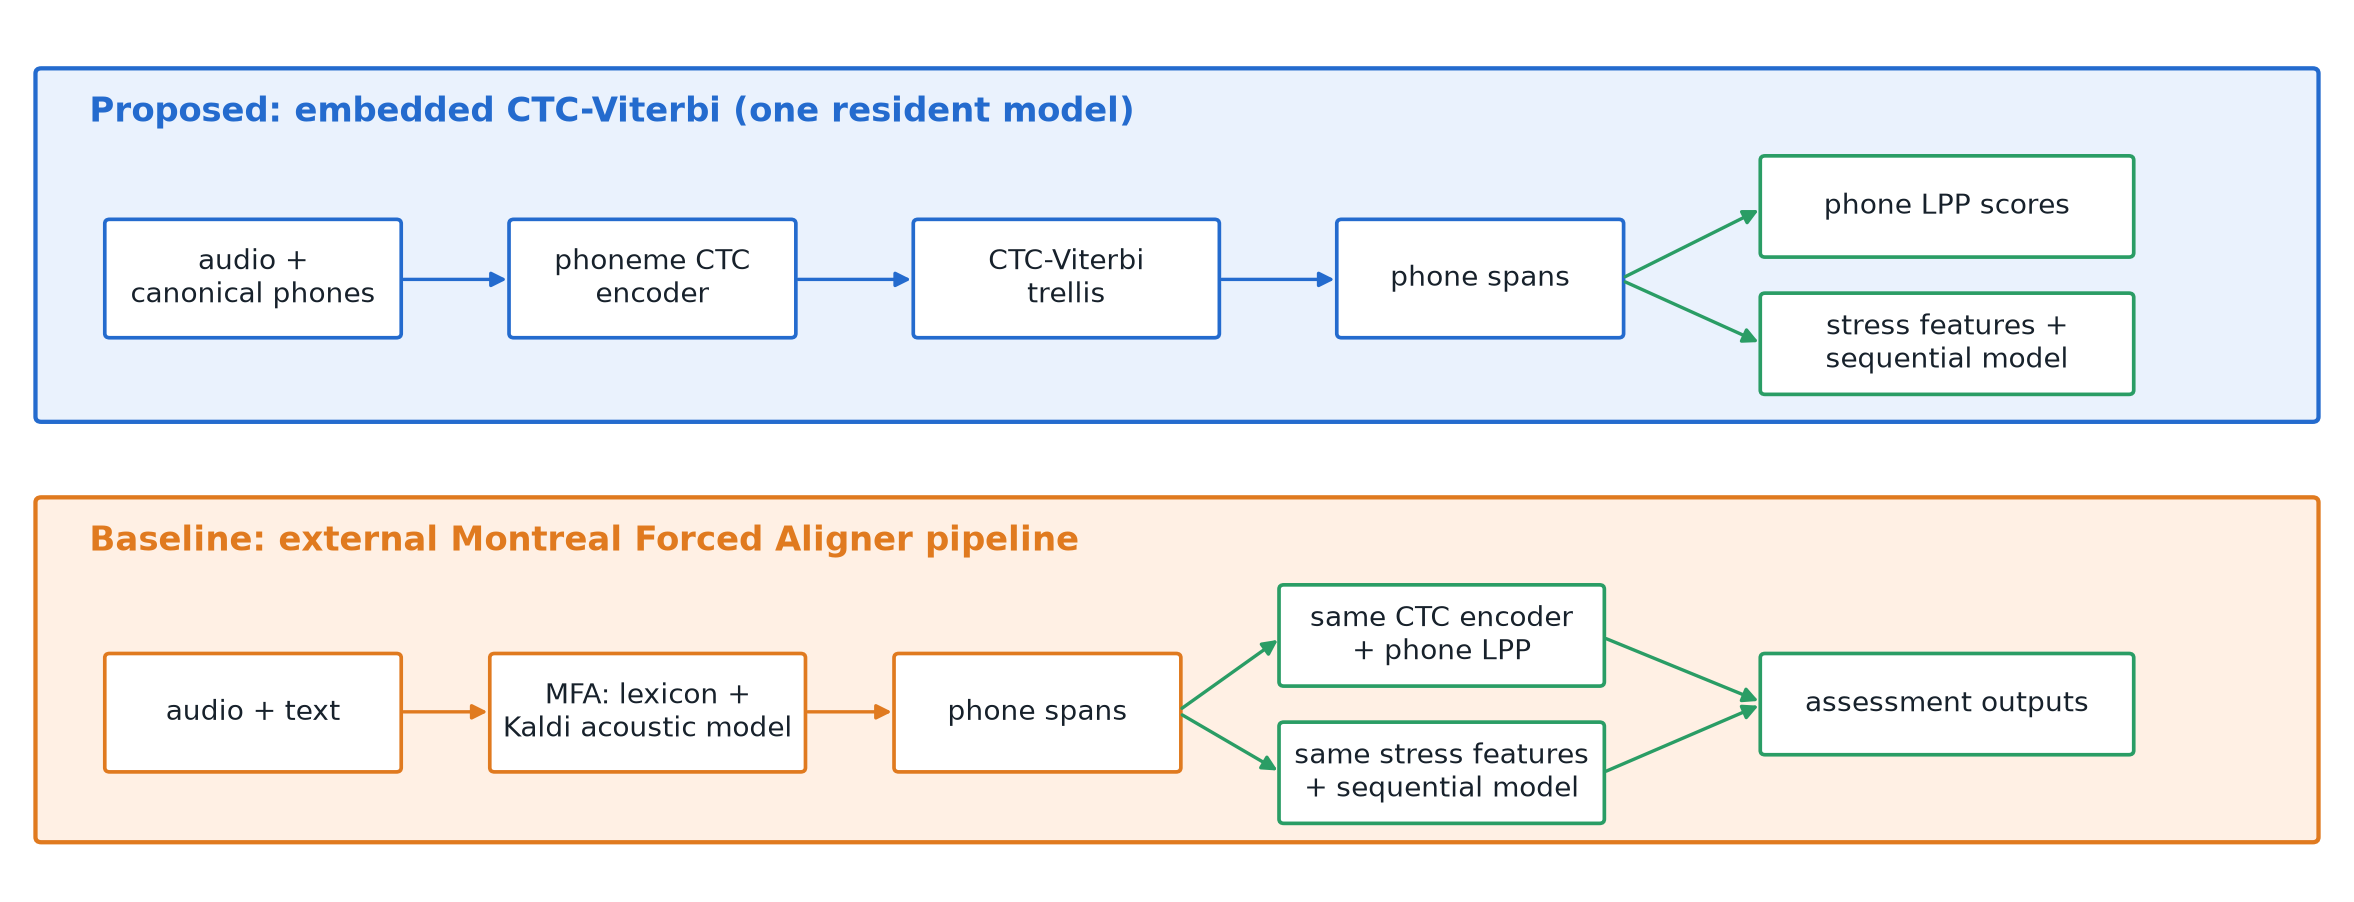
\includegraphics[width=0.98\textwidth]{fig_architecture.png}
    \caption{The proposed path obtains phone scores and stress regions from one
    resident CTC model. The baseline first runs external MFA, then passes its
    intervals to the same CTC score and stress modules.}
    \label{fig:architecture}
\end{figure*}

\section{Related Work}

Witt and Young introduced phone-level pronunciation confidence for language
learning~\cite{witt2000phone}; later DNN-GOP formulations replaced generative
likelihoods with neural posteriors~\cite{hu2015improved}. SpeechOcean762's
released Kaldi recipe constructs an alignment graph directly from the
expert-selected canonical phone sequence and fits phone-specific regressors
~\cite{zhang2021speechocean762}. Cao et al. show that CTC also supports
alignment-marginalized scalar and vector GOP definitions~\cite{cao2024framework}.
Our objective differs: we deliberately recover a single CTC path because both
phone scoring and stress feature extraction require localized evidence, while
eliminating a separate aligner service.

Lexical stress is conveyed by relative duration, intensity, and fundamental
frequency~\cite{fry1958experiments}. Yarra et al. demonstrate that automatic
boundary quality affects stress detection and examine forced-alignment acoustic
models and lexicons on ISLE~\cite{yarra2019comparison}. Mallela et al. treat a
word as a sequence of syllable features, use masking for variable-length words,
and compare RNN, LSTM, GRU, and attention models on German and Italian learners
in ISLE~\cite{mallela2024comparative}. Their pipeline obtains phone alignments
automatically, manually corrects them, derives syllables, and applies a
word-level post-processing rule that selects one primary stress. We reuse the
sequential and word-constraint ideas, but our local checkpoint and feature code
are an adaptation rather than a reproduction of their ISLE model.

\section{Method}

\subsection{Embedded CTC--Viterbi path}

Let $\mathbf{L}=(l_1,\ldots,l_U)$ be the expected phone sequence and let
$\ell_{t,k}=\log p(k\mid\mathbf{x},t)$ be the log posterior for token $k$ at
CTC frame $t$. We form the expanded state sequence
\begin{equation}
\mathbf{z}=(\phi,l_1,\phi,l_2,\ldots,\phi,l_U,\phi),
\end{equation}
where $\phi$ is blank. The Viterbi recurrence is
\begin{equation}
V_t(s)=\ell_{t,z_s}+\max_{r\in\mathcal{P}(s)}V_{t-1}(r),
\label{eq:viterbi}
\end{equation}
where $\mathcal{P}(s)$ permits staying at $s$, advancing from $s-1$, and
advancing from $s-2$ into a phone state only when the skipped and current
phone labels differ. The last restriction forces repeated adjacent phones to
pass through blank. Initialization permits the leading blank or first phone;
termination permits the last phone or trailing blank. Backtracking yields one
state per frame in $\mathcal{O}(TU)$ time and $\mathcal{O}(TU)$ memory.

The implementation is verified against exhaustive enumeration of every valid
path in small lattices. It also includes a dedicated repeated-phone test.

\subsection{Phone regions and score}

Let $F_i=\{t:z_{s_t}=l_i\}$ be the frames assigned to phone $i$. Its scalar
score is the frame-averaged log posterior
\begin{equation}
g_i=\frac{1}{|F_i|}\sum_{t\in F_i}\ell_{t,l_i}.
\label{eq:lpp}
\end{equation}
For a continuous interval, the start and end of the phone-state run are
extended across adjacent blank gaps by midpoint splitting. Equation
~\ref{eq:lpp} uses only phone-state frames, whereas the expanded intervals are
passed to the stress branch.

For the MFA baseline, MFA supplies phone intervals. Frame centers falling
inside an MFA interval replace $F_i$ in Eq.~\ref{eq:lpp}; a nearest-frame rule
handles an interval shorter than one CTC frame. A global edit-distance match
pairs identical phones between the expert canonical sequence and the MFA
output. Only phones matched in both conditions enter the comparison.

\subsection{Stress scoring}

Canonical pronunciations are syllabified by the maximal-onset principle. Phone
regions are grouped by syllable and the vowel-phone interval defines the
nucleus. The local feature extractor emits 19 acoustic measurements covering
duration, pitch, intensity, and spectral properties and 19 context features.
The fixed scorer contains three LSTM layers (64, 32, and 16 units), a
four-unit attention projection, and a sigmoid output. Its standardized neural
scores are combined with a relative acoustic-prominence score; word-level
argmax selects exactly one primary-stress location. This same scorer, scaler,
audio, pronunciation, and post-processing are used for CTC and MFA intervals.

\section{Experimental Design}

\subsection{Corpus and models}

SpeechOcean762 contains 5,000 English utterances from 250 Mandarin-speaking
learners, divided into speaker-disjoint sets of 2,500 utterances from 125
speakers each~\cite{zhang2021speechocean762}. Five experts supply phone
accuracy scores from 0 to 2 and word stress scores: 10 for correct stress (or a
monosyllable) and 5 for incorrect stress. We retain the official split.

The resident model is
\texttt{mostafaashahin/wav2vec2-base-timit-phoneme-arpa-39}, a Wav2Vec~2.0
base CTC phone model~\cite{baevski2020wav2vec}. MFA 3.4.2 uses its
\texttt{english\_us\_arpa} dictionary and acoustic model. With
\texttt{--ignore\_oovs}, MFA exports 2,462 training and 2,447 test TextGrids.
The paired phone sets contain 43,594 training and 43,613 test phones. The CTC
system itself scores all 2,500 test utterances; restriction is required only
for the paired baseline comparison.

\subsection{Phone endpoint}

For each condition, phone-specific quadratic regressors map Eq.~\ref{eq:lpp}
to the human grade. Regressors are fitted only on the matched official training
phones; a global quadratic is used if a phone has fewer than 20 examples.
Predictions are clipped to $[0,2]$. We report Pearson correlation (PCC) and
Spearman correlation (SRCC) on the paired test phones. To preserve dependence
within a speaker, the central PCC difference is evaluated with 2,000 paired
speaker bootstrap samples.

\subsection{Stress endpoints}

The stress comparison includes polysyllabic words whose complete phone sequence
is matched to MFA, yielding 1,621 words: 1,575 rated correct and 46 rated as
stress errors. The primary boundary-sensitivity endpoint is canonical
stress-location accuracy among human-correct words; here the expert label
establishes that the realized stress should agree with the dictionary location.
We bootstrap its paired CTC-minus-MFA difference by speaker 2,000 times. As a
secondary endpoint, the predicted probability assigned to the canonical
primary syllable is used to distinguish human-correct from human-incorrect
stress, reported as area under the ROC curve (AUROC). SpeechOcean does not
annotate the realized destination of a misplaced stress, so wrong-location
accuracy cannot be measured for the 46 errors.

\subsection{Latency protocols}

All timings use the same ARM64 macOS CPU and a complete paired batch workload.
For each of the 2,447 MFA-aligned test utterances, both conditions execute one
resident CTC encoding, score the same matched phone tokens, and run the same
stress model on every fully matched polysyllabic word. The proposed condition
additionally runs the CTC--Viterbi trellis; the baseline uses an MFA TextGrid.
Condition order alternates by utterance after one excluded warm-up to reduce
systematic order and thermal effects. Each condition uses one top-level Python
assessment process and the same four PyTorch intra-operation CPU threads.

The baseline is also charged for a fresh MFA 3.4.2 corpus alignment with
\texttt{--num\_jobs 1}. This stage processes all 2,500 inputs, including the 53
cases for which no TextGrid is exported, and takes 89.3 s. Complete serial wall
time is the measured MFA alignment time plus measured downstream assessment
time. We divide each condition's total by the 2,447 paired outputs. This design
tests the deployed assessment workload rather than alignment-only throughput.

\section{Results}

\begin{table}[t]
\centering
\caption{Paired phone assessment on 43,613 held-out phones.}
\label{tab:phone}
\begin{tabular}{lrr}
\toprule
Metric & CTC--Viterbi & MFA \\
\midrule
Raw PCC & 0.401 & 0.216 \\
Raw SRCC & 0.325 & 0.233 \\
Quadratic PCC & \textbf{0.459} & 0.317 \\
Quadratic SRCC & \textbf{0.376} & 0.302 \\
\bottomrule
\end{tabular}
\end{table}

Table~\ref{tab:phone} shows higher phone correlation for CTC--Viterbi. The
paired PCC difference is 0.142, with a 95\% speaker-bootstrap interval of
[0.120, 0.164]. Since the interval lies above zero, the result establishes no
observed accuracy trade-off and favors the embedded regions under this
protocol. CTC and MFA boundaries differ by 50.0 ms median; mean disagreement is
150.7 ms because a minority of alignments have large offsets.

\begin{table}[t]
\centering
\caption{Paired stress results on 1,621 polysyllabic words.}
\label{tab:stress}
\begin{tabular}{lrr}
\toprule
Metric & CTC--Viterbi & MFA \\
\midrule
Canonical location accuracy$^\dagger$ & \textbf{74.9\%} & 69.5\% \\
Correct-stress AUROC & \textbf{0.726} & 0.695 \\
Grade PCC & \textbf{0.155} & 0.133 \\
Grade SRCC & \textbf{0.144} & 0.122 \\
\bottomrule
\multicolumn{3}{l}{\footnotesize $^\dagger$Among 1,575 words rated correct by humans.}
\end{tabular}
\end{table}

For canonical stress location (Table~\ref{tab:stress}), the paired difference
is 5.4 percentage points and the 95\% speaker-bootstrap interval is [2.8, 8.0]
points. Correct-stress discrimination also favors CTC descriptively. Because
only 46 paired polysyllabic words carry the error grade, AUROC and grade
correlations should be treated as secondary, high-variance estimates.

\begin{table}[t]
\centering
\caption{Mean complete-pipeline latency per paired utterance. MFA alignment is
the one-job corpus wall time amortized over 2,447 outputs.}
\label{tab:latency}
\begin{tabular}{lrrr}
\toprule
Component & CTC--Viterbi & MFA & MFA/CTC \\
\midrule
CTC encoding & 62.9 ms & 62.8 ms & --- \\
Phone regions + LPP & 4.4 ms & 0.2 ms & --- \\
Stress branch & 31.3 ms & 29.4 ms & --- \\
External alignment & --- & 36.5 ms & --- \\
\textbf{Complete pipeline} & \textbf{98.6 ms} & 128.8 ms & \textbf{1.31$\times$} \\
\bottomrule
\end{tabular}
\end{table}

Table~\ref{tab:latency} shows that the embedded path is 1.31$\times$ faster for
the complete matched workload. CTC--Viterbi region construction costs more than
reading and indexing existing MFA intervals, but it replaces the 89.3-s
external alignment stage. The two encodings are nearly identical in cost, as
expected, and the same stress workload is executed in both conditions. An
exploratory four-job MFA run reached 28.0 ms per input for alignment alone;
because it excludes the shared CTC phone scorer and stress branch, it is not
used as the end-to-end comparison. The speed claim remains specific to this
hardware, worker configuration, and corpus.

\section{Discussion and Limitations}

The result suggests that a CTC model trained to recognize phones can localize
the evidence most useful to its own posterior score better than cross-system
MFA intervals. This does not imply that its timestamps are closer to manual
articulatory boundaries. MFA is the reference pipeline, not ground truth, and
the median 50-ms disagreement cannot decide which boundary is physically
correct. The experiment instead asks an application-level question: which
interval source yields better human-correlated assessments when downstream
components are held fixed?

The paired design removes many confounds but has limitations. MFA OOV failures
exclude 38 training and 53 test utterances. Global phone-sequence matching
removes unmatched tokens from both conditions, potentially favoring easier
examples. The CTC acoustic model was trained for TIMIT-style phone recognition,
not specifically for L2 assessment. The quadratic calibration may not transfer
to another learner population. An external-aligner baseline using a native
phone model matched more closely to the CTC inventory could perform differently.

The stress experiment validates a boundary substitution in the repository's
fixed Mallela-inspired scorer; it does not reproduce Mallela et al.'s manually
corrected ISLE experiment. SpeechOcean supplies only correct/incorrect word
stress, not the realized wrong stress location. A future study should repeat
the paired comparison on ISLE with speaker-disjoint German/Italian folds,
manual syllable boundaries, and explicit wrong-location labels. Finally, a
parallel MFA deployment and a batched or parallel CTC service could change
throughput; worker-count scaling should be measured separately rather than
mixed into the one-job method comparison.

Terminology also deserves care. Some authors use \emph{forced alignment} for
any transcript-conditioned best path, including Eq.~\ref{eq:viterbi}. Our
engineering distinction is between an embedded path in the assessment model
and the external MFA/Kaldi pipeline. Accordingly, the strongest portable terms
for the proposal are \emph{MFA-free} and \emph{external-aligner-free}.

\section{Conclusion}

We replaced peak timing and the external alignment dependency with one
canonical-conditioned CTC--Viterbi path shared by phoneme GOP and lexical-stress
assessment. On paired SpeechOcean762 data, the embedded path improves both
phone correlation and canonical stress-location accuracy relative to MFA
regions, with speaker-bootstrap intervals excluding an accuracy loss. It also
reduces complete one-job phone-and-stress processing time from 128.8 to 98.6 ms
per paired utterance. The proposed architecture is therefore a faster
single-model path under the measured protocol, not a universal claim about all
hardware, worker counts, acoustic models, or corpora.

\bibliographystyle{IEEEtran}
\bibliography{references}

\end{document}
